\chapter{object list}
\label{sec:object_list}
\lhead[tempest 2000]{}
\lstset{style=68KStyle}
About 60 times a second the Jaguar will want to write something to the screen. A 
module in the Jaguar system called the 'Object Processor' will take whatever the current list of things
to draw happens to be and draw them. It's Tempest 2000's job to keep this beast well fed
with new stuff. The way to do this is to keep shovelling fresh imagery into a structure
called an 'Object List' for the Object Processor to chew on. As the name suggests this is a list of objects, but since everything
is an object these days we might need to be more specific about what these objects are and
what they contain.

There are a few different types of objects, but the only one of real interest is the 
one that contains something that can be displayed: an image. This image takes the form of
a section of data similar to the cry pixel data we looked at in 'cry if i want to'. There
can be a number of different flavours of this data that make the Object Processor's job easier
in different circumstances but in Tempest 2000 we only ever detain ourselves with the
rich cry data, the good stuff.

Below we set out the raw contents of an actual Object List used for a single frame in the
'Demo' sequence. The interesting objects in the list are the 'Bit Mapped Objects'. You can
tell they're interesting because we have to specify so much about them that we need two 'phrases'
(i.e. two sets of 8 bytes each) to encapsulate it all.

\begin{figure}[H]
  {
    \setlength{\tabcolsep}{3.0pt}
    \setlength\cmidrulewidth{\heavyrulewidth} % Make cmidrule = 
    \begin{adjustbox}{center}
      \begin{tabular}[t]{ll}
        \toprule
        Data & Object Type\\
        \midrule
        \icode{13,48,00,1D,6E,45,C1,60}
        &
        Bit Mapped Object (First Phrase)
        \\
        \icode{00,00,80,06,01,80,CF,F8}
        &
        Bit Mapped Object (Second Phrase)
        \\
        \icode{00,00,00,00,00,00,00,04}
        &
        Stop Object
        \\
        \icode{00,00,00,00,00,00,00,04}
        &
        Stop Object
        \\
        \icode{05,00,00,1D,72,0C,01,E0}
        &
        Bit Mapped Object (First Phrase)
        \\
        \icode{00,00,80,06,01,80,CF,F8}
        &
        Bit Mapped Object (Second Phrase)
        \\
        \bottomrule
      \end{tabular}
    \end{adjustbox}
  }\caption{Object List}
\end{figure}

It is kind of amazing how much you can pack into 16 bytes if you try. Below we parse out the contents
of the first 'Bit Mapped Object' in our Object List and show the screen of pixel data it references
in the first 8-byte phrase.

\begin{figure}[H]
  {
    \setlength{\tabcolsep}{3.0pt}
    \setlength\cmidrulewidth{\heavyrulewidth} % Make cmidrule = 
    \begin{adjustbox}{center}
      \begin{tabular}[t]{lll}
        \toprule
        Raw Data & Parsed Data & Image at \icode{DATA: 0x134800} \\
        \midrule
          \tcode{13,48,00,1D,6E,45,C1,60}
        &
        \makecell[tl]{
          \begingroup
          \renewcommand{\arraystretch}{.8} % Default value: 1
          \begin{tabular}[t]{ll}
            \tcode{TYPE: 0}   &    \tcode{LINK: 0xeb70}  \\
            \tcode{YPOS: 44} &     \tcode{DATA: 0x134800}  \\
            \tcode{HEIGHT: 279} &  \\
            \tcode{} &  \\
            \tcode{} &  \\
          \end{tabular}
          \endgroup
        } &
        \multirow{2}{*}[0.1cm]{
          \makecell[tl]{
            \includegraphics[height=4.2cm]{object_list/data_1.png}%
          }
        } \\
        \addlinespace
          \tcode{00,00,80,06,01,80,CF,F8}
        &
        \makecell[tl]{
          \begingroup
          \renewcommand{\arraystretch}{.8} % Default value: 1
          \begin{tabular}[t]{ll}
            \tcode{XPOS: -7   } &  \tcode{REFLECT: 0}  \\
            \tcode{DEPTH: 4} &    \tcode{RMW: 0}  \\
            \tcode{PITCH: 1} &    \tcode{TRANS: 1}  \\
            \tcode{DWIDTH: 96} &  \tcode{RELEASE: 0}  \\
            \tcode{IWIDTH: 96} &  \tcode{FIRSTPIX: 0}  \\
            \tcode{INDEX: 0} & \\
          \end{tabular}
          \endgroup
        } &
        \\
        \bottomrule
      \end{tabular}
    \end{adjustbox}
  }\caption{First Bit Mapped Object in the Object List}
\end{figure}

Here is what a selection of the parameters we supply above are a way of saying:

\begin{figure}[H]
  {
    \setlength{\tabcolsep}{3.0pt}
    \setlength\cmidrulewidth{\heavyrulewidth} % Make cmidrule = 
    \begin{adjustbox}{center}
      \begin{tabular}[t]{lll}
        \icode{DATA: 0x134800}
        &
        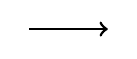
\begin{tikzpicture}
          \draw[->,line width=1pt] (0,0) to (1,0);
        \end{tikzpicture}
        &
        Paint the data found at address \icode{0x134800} in RAM. 
        \\
        \icode{DEPTH: 4}
        &
        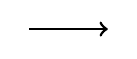
\begin{tikzpicture}
          \draw[->,line width=1pt] (0,0) to (1,0);
        \end{tikzpicture}
        &
        Treat the data as using 16 bits for each pixel. 
        \\
        \icode{YPOS: 44}
        &
        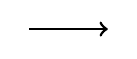
\begin{tikzpicture}
          \draw[->,line width=1pt] (0,0) to (1,0);
        \end{tikzpicture}
        &
        Start painting this image at line 44.
        \\
        \icode{XPOS: -7}
        &
        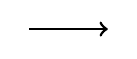
\begin{tikzpicture}
          \draw[->,line width=1pt] (0,0) to (1,0);
        \end{tikzpicture}
        &
        Start painting this image at X pos -7.
        \\
        \icode{DWIDTH: 96}
        &
        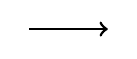
\begin{tikzpicture}
          \draw[->,line width=1pt] (0,0) to (1,0);
        \end{tikzpicture}
        &
        Treat the data as having a line width of 380 (96*4).
        \\
        \icode{IWIDTH: 96}
        &
        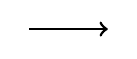
\begin{tikzpicture}
          \draw[->,line width=1pt] (0,0) to (1,0);
        \end{tikzpicture}
        &
        Treat the image as having a width of 380 (96*4).
        \\
        \icode{HEIGHT: 279}
        &
        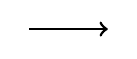
\begin{tikzpicture}
          \draw[->,line width=1pt] (0,0) to (1,0);
        \end{tikzpicture}
        &
        Treat the data as having a height of 280 lines.
        \\
      \end{tabular}
    \end{adjustbox}
  }
\end{figure}

You'll notice we have what looks like a lovely bit of glitch at the bottom of our image data.

\begin{figure}[H]
    \centering
    \begin{adjustbox}{width=11cm,center}
      \frame{\includegraphics[width=12cm]{src/object_list/data_1_glitch.png}}%
    \end{adjustbox}
\end{figure}

This handsome scramble is the left-over data from previously drawn frames in the RAM. It
is not visible because as we noted above we are painting this image at Y position 49, so
although we are painting the full 280 lines of data only the first 231 are visible, and
our glorious glitch sits off screen.

These vacant 49 lines at the top of the screen are occupied by our second 'Bit Mapped Object'.
This is the player's score and their remaining lives:

\begin{figure}[H]
  {
    \setlength{\tabcolsep}{3.0pt}
    \setlength\cmidrulewidth{\heavyrulewidth} % Make cmidrule = 
    \begin{adjustbox}{center}
      \begin{tabular}[t]{lll}
        \toprule
        Raw Data & Parsed Data & Image in Data \icode{0x134800} \\
        \midrule
        \tcode{05,00,00,1D,72,0C,01,E0}
        &
        \makecell[tl]{
          \begingroup
          \renewcommand{\arraystretch}{.8} % Default value: 1
          \begin{tabular}[t]{ll}
            \tcode{TYPE: 0}   &    \tcode{LINK: 0xeb90}  \\
            \tcode{YPOS: 60} &     \tcode{DATA: 0x50000}  \\
            \tcode{HEIGHT: 48 } &  \\
          \end{tabular}
          \endgroup
        } &
        \multirow{2}{*}[-1.1cm]{
          \makecell[tl]{
            \includegraphics[height=1.2cm]{object_list/data_4.png}%
          }
        } \\
        \tcode{00,00,80,06,01,80,CF,F8}
        &
        \makecell[tl]{
          \begingroup
          \renewcommand{\arraystretch}{.8} % Default value: 1
          \begin{tabular}[t]{ll}
            \tcode{XPOS: -7   } &  \tcode{REFLECT: 0}  \\
            \tcode{DEPTH: 4} &    \tcode{RMW: 0}  \\
            \tcode{PITCH: 1} &    \tcode{TRANS: 1}  \\
            \tcode{DWIDTH: 96} &  \tcode{RELEASE: 0}  \\
            \tcode{IWIDTH: 96} &  \tcode{FIRSTPIX: 0}  \\
            \tcode{INDEX: 0} & \\
          \end{tabular}
          \endgroup
        } &
        \\
        \bottomrule
      \end{tabular}
    \end{adjustbox}
  }\caption{Second Bit Mapped Object in the Object List}
\end{figure}

We can be flexible about how many Bit Mapped Objects we have and even what we put in them.
Here are the two objects we use for the high score screen. The first is the rotating web
in the background:

\begin{figure}[H]
  {
    \setlength{\tabcolsep}{3.0pt}
    \setlength\cmidrulewidth{\heavyrulewidth} % Make cmidrule = 
    \begin{adjustbox}{center}
      \begin{tabular}[t]{lll}
        \toprule
        Raw Data & Parsed Data & Image at \icode{DATA: 0x100000} \\
        \midrule
          \tcode{10,00,00,1D,6E,45,C1,60}
        &
        \makecell[tl]{
          \begingroup
          \renewcommand{\arraystretch}{.8} % Default value: 1
          \begin{tabular}[t]{ll}
            \tcode{TYPE: 0}   &    \tcode{LINK: 0xeb70}  \\
            \tcode{YPOS: 44} &     \tcode{DATA: 0x100000}  \\
            \tcode{HEIGHT: 279} &  \\
            \tcode{} &  \\
            \tcode{} &  \\
          \end{tabular}
          \endgroup
        } &
        \multirow{2}{*}[0.1cm]{
          \makecell[tl]{
            \includegraphics[height=4.2cm]{object_list/data_1_hiscore.png}%
          }
        } \\
        \addlinespace
          \tcode{00,00,80,06,01,80,CF,F8}
        &
        \makecell[tl]{
          \begingroup
          \renewcommand{\arraystretch}{.8} % Default value: 1
          \begin{tabular}[t]{ll}
            \tcode{XPOS: -7   } &  \tcode{REFLECT: 0}  \\
            \tcode{DEPTH: 4} &    \tcode{RMW: 0}  \\
            \tcode{PITCH: 1} &    \tcode{TRANS: 1}  \\
            \tcode{DWIDTH: 96} &  \tcode{RELEASE: 0}  \\
            \tcode{IWIDTH: 96} &  \tcode{FIRSTPIX: 0}  \\
            \tcode{INDEX: 0} & \\
          \end{tabular}
          \endgroup
        } &
        \\
        \bottomrule
      \end{tabular}
    \end{adjustbox}
  }
\end{figure}

The second is the high-score screen itself:

\begin{figure}[H]
  {
    \setlength{\tabcolsep}{3.0pt}
    \setlength\cmidrulewidth{\heavyrulewidth} % Make cmidrule = 
    \begin{adjustbox}{center}
      \begin{tabular}[t]{lll}
        \toprule
        Raw Data & Parsed Data & Image at \icode{DATA: 0x5000} \\
        \midrule
          \tcode{05,00,00,1D,72,45,C1,60}
        &
        \makecell[tl]{
          \begingroup
          \renewcommand{\arraystretch}{.8} % Default value: 1
          \begin{tabular}[t]{ll}
            \tcode{TYPE: 0}   &    \tcode{LINK: 0xeb90}  \\
            \tcode{YPOS: 44} &     \tcode{DATA: 0x5000}  \\
            \tcode{HEIGHT: 279} &  \\
            \tcode{} &  \\
            \tcode{} &  \\
          \end{tabular}
          \endgroup
        } &
        \multirow{2}{*}[0.1cm]{
          \makecell[tl]{
            \includegraphics[height=4.2cm]{object_list/data_4_hiscore.png}%
          }
        } \\
        \addlinespace
          \tcode{00,00,80,06,01,80,CF,F8}
        &
        \makecell[tl]{
          \begingroup
          \renewcommand{\arraystretch}{.8} % Default value: 1
          \begin{tabular}[t]{ll}
            \tcode{XPOS: -7   } &  \tcode{REFLECT: 0}  \\
            \tcode{DEPTH: 4} &    \tcode{RMW: 0}  \\
            \tcode{PITCH: 1} &    \tcode{TRANS: 1}  \\
            \tcode{DWIDTH: 96} &  \tcode{RELEASE: 0}  \\
            \tcode{IWIDTH: 96} &  \tcode{FIRSTPIX: 0}  \\
            \tcode{INDEX: 0} & \\
          \end{tabular}
          \endgroup
        } &
        \\
        \bottomrule
      \end{tabular}
    \end{adjustbox}
  }
\end{figure}

Notice that unlike our previous case we are superimposing these two images (or compositing them)
so that the high score appears above the rotating web.
